The scattering particle track from focal plane need to be reconstructed to the target before bended by the spectrometer magnets to determine the scattering vertex, scattering angle and momentum. To do this , a magnet optics matrix need to be well calibrated.
\section{Corrdinate system}
There are two coordinate system are important for the reconstructed variable: The Hall Coordinate System(HCS) and the Target Coordinate System(TCS). The origin of the HCS is at the Hall center.  Z axis direction is alone the beam line and point to the beam dump and y axis is point horizontally up. Each HRS also has its own TCS(Fig \ref{optics_plt1} . The z axis of the TCS is along the center ray of the spectrometer and the x axis is horizontally pointing down. The original of the TCS is at a constant distance   $L$ in front of the HRS entrance and this distance is defined with the distance from Hall center to the HRS entrance under the ideal situation which means the all the spectrometer offsets are zero. According to this definition, we can see that under the ideal case, the origin of the TCS can match the origin of the HCS. The trajectory of the scattering particle can be reocnstructed to the target described by 4 variables in the TCS: the position in the no dispersive plane($y_{tg}$), the angles in the dispersive direction(out-of-plan, $\theta_{tg}$) and the non-dispersive direction(in-plane, $\phi_{tg}$) and the relative momentum $\delta=(p-p_{0})/p_{0}$, where the $p$ is the momentum for the scattering momentum and $p_{0}$ is the setting momentum of the HRS.
\begin{figure}
 	\begin{center}
 		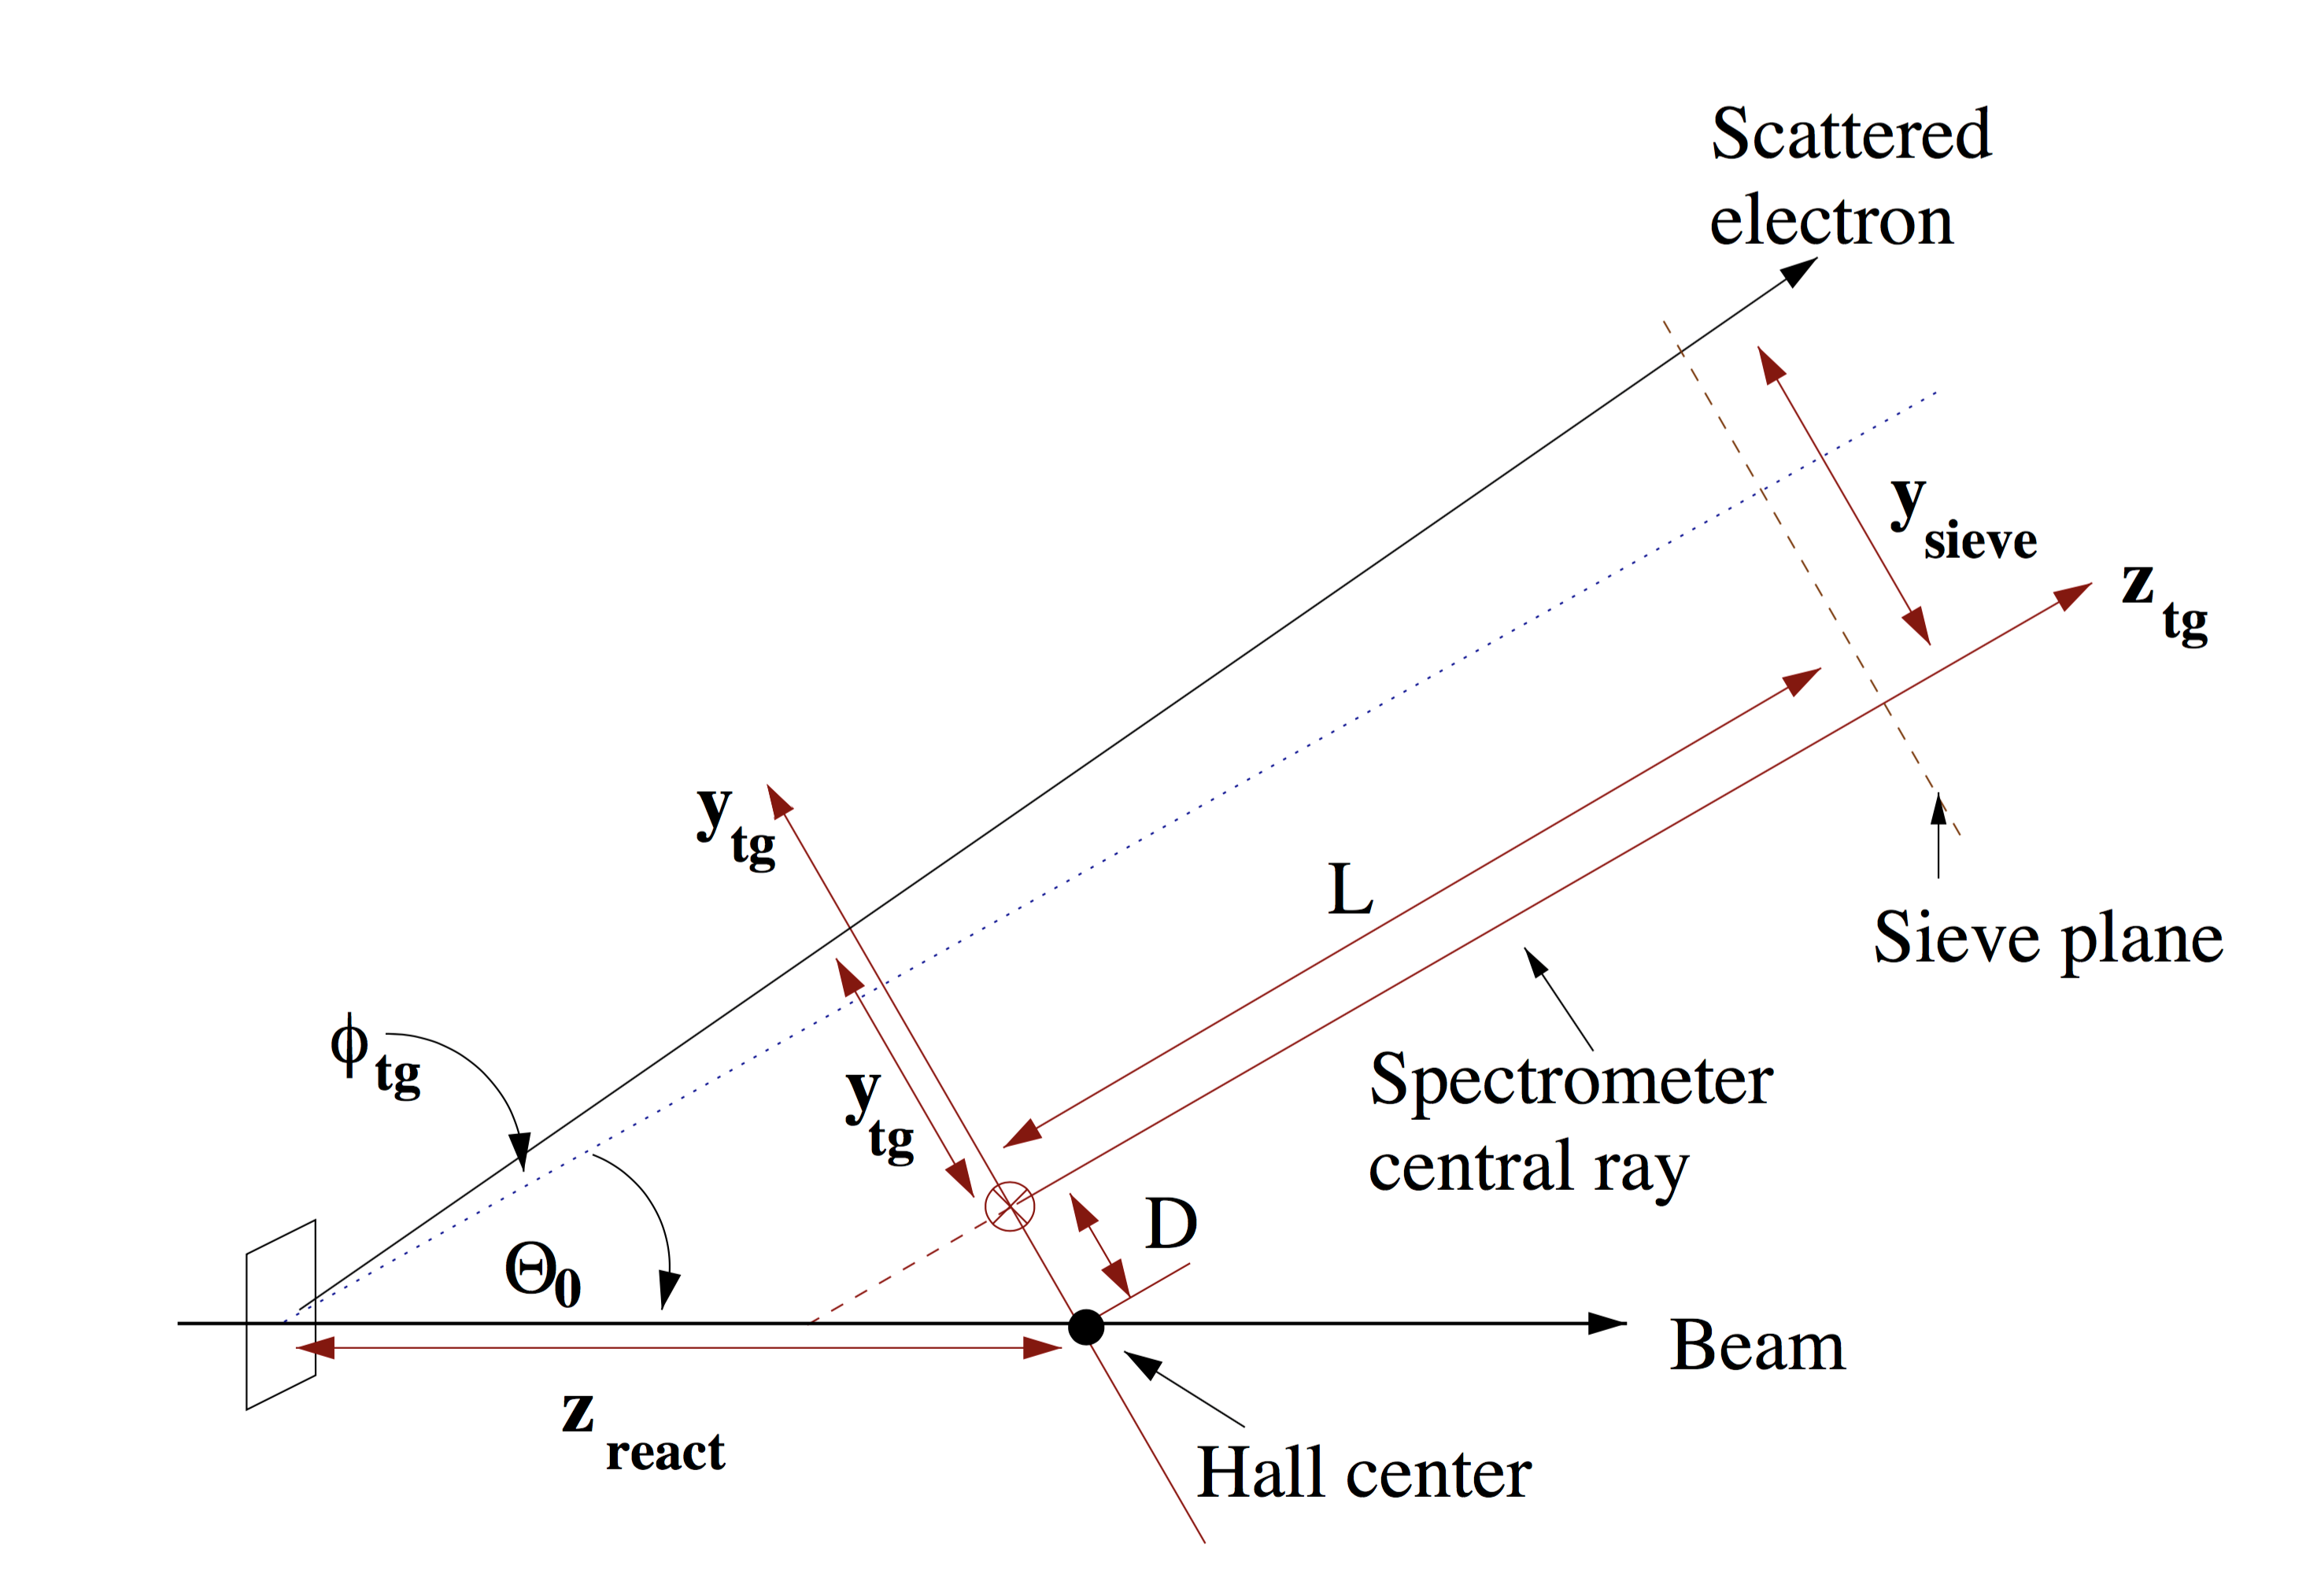
\includegraphics[width=0.2\textwidth] {./optics_plot/optics_4.png}
 		\caption{The schematic plot of the TCS from RefXXX, in which D stands for the spectrmoeter offset from the hall center } \label{optics_plt1}
 	\end{center}
\end{figure}   



The relations between the 4 traking variables in the focal plane and the 4 reconstrcuted variables at TCS can be described as a set of the following polynomials:
\begin{equation}  
\left\{  
             \begin{array}{lr}  
             y_{tg}=\sum_{jkl}Y_{jkl} \theta_{fp}^{j} y_{fp}^{k} \phi_{fp}^{l} \\  
             \theta_{tg}=\sum_{jkl}T_{jkl} \theta_{fp}^{j} y_{fp}^{k} \phi_{fp}^{l} \\    
             \phi_{tg}=\sum_{jkl}P_{jkl} \theta_{fp}^{j} y_{fp}^{k} \phi_{fp}^{l} \\     
             \delta_{tg}=\sum_{jkl}D_{jkl} \theta_{fp}^{j} y_{fp}^{k} \phi_{fp}^{l}\\  
             \end{array}  
\right.  
\label{optics_1}
\end{equation}  
where the 4 sets of cofficients are the function of $x_{fp}$:
\begin{equation}  
\left\{  
             \begin{array}{lr}  
             Y_{jkl}=\sum_{i=0}^{m} C_{ijkl}^{Y} x_{fp}^{i} \\  
             T_{jkl}=\sum_{i=0}^{m} C_{ijkl}^{T} x_{fp}^{i} \\
             P_{jkl}=\sum_{i=0}^{m} C_{ijkl}^{P} x_{fp}^{i} \\
             D_{jkl}=\sum_{i=0}^{m} C_{ijkl}^{D} x_{fp}^{i} \\ 
             \end{array}  
\right.  
\label{optics_2 }
\end{equation} 
The four sets of cofficients $C_{ijkl}^{Y/T/P/D}$ describe the optics properties of the spectrometer magnets and the above four sets of polynmoinal also called the HRS optics matrix.                                                                     
\section{Optics Data Taking and Optimized Procedure }
The so-called optics calibration is that to determine the cofficients described in Eq \ref{optics_2 }. In order to reach this goal, some desigined data need to be taking during druring the experiment. Since the 4 sets of the matrice are independent mathematically, in principle, we can use different sets of data to calibrate different target variable . Experimentally, $C^{Y}$, $C^{T}$ and $C^{P}$ use one set of the data which is expected can cover the spectrometer acceptance as much as it can and for inclusive experiment, $C_{P}$ can only choose the kinematics setting with the well known scattering momentum such as the elastic scattering data. To label the spatial variables in the TCS, a mutifoil target (Fig \ref{optics_plt2} ) and a sieve-slit collimator (Fig \ref{optics_plt3})  are used for the optics calibration data. For Tritium Experiment, the mutifoil target is consisted of 11 carbon foil which are evenlty arranged along the beam direction. The distance between the two adjacent foils is 2.5cm and the total length of the mutifoil target is 25cm which is equivalent to the gas target length. The sieve-slit collimater tritium used is the new desgined one from the GMP experiment which is make of tungsten with 1in thickness. Electrons will lose enough energy   by passing through the tungsten, so that only electrons go throught the hole can reach the focal plane.  In addition, a complete and percise survey which including the postion of the spectrometer, target and sieve-slit also import to label data correctly. Not only that, a well understanded beam positon from a calibrated BPMs also to do the optics calibration.

\begin{figure}
 	\begin{center}
 		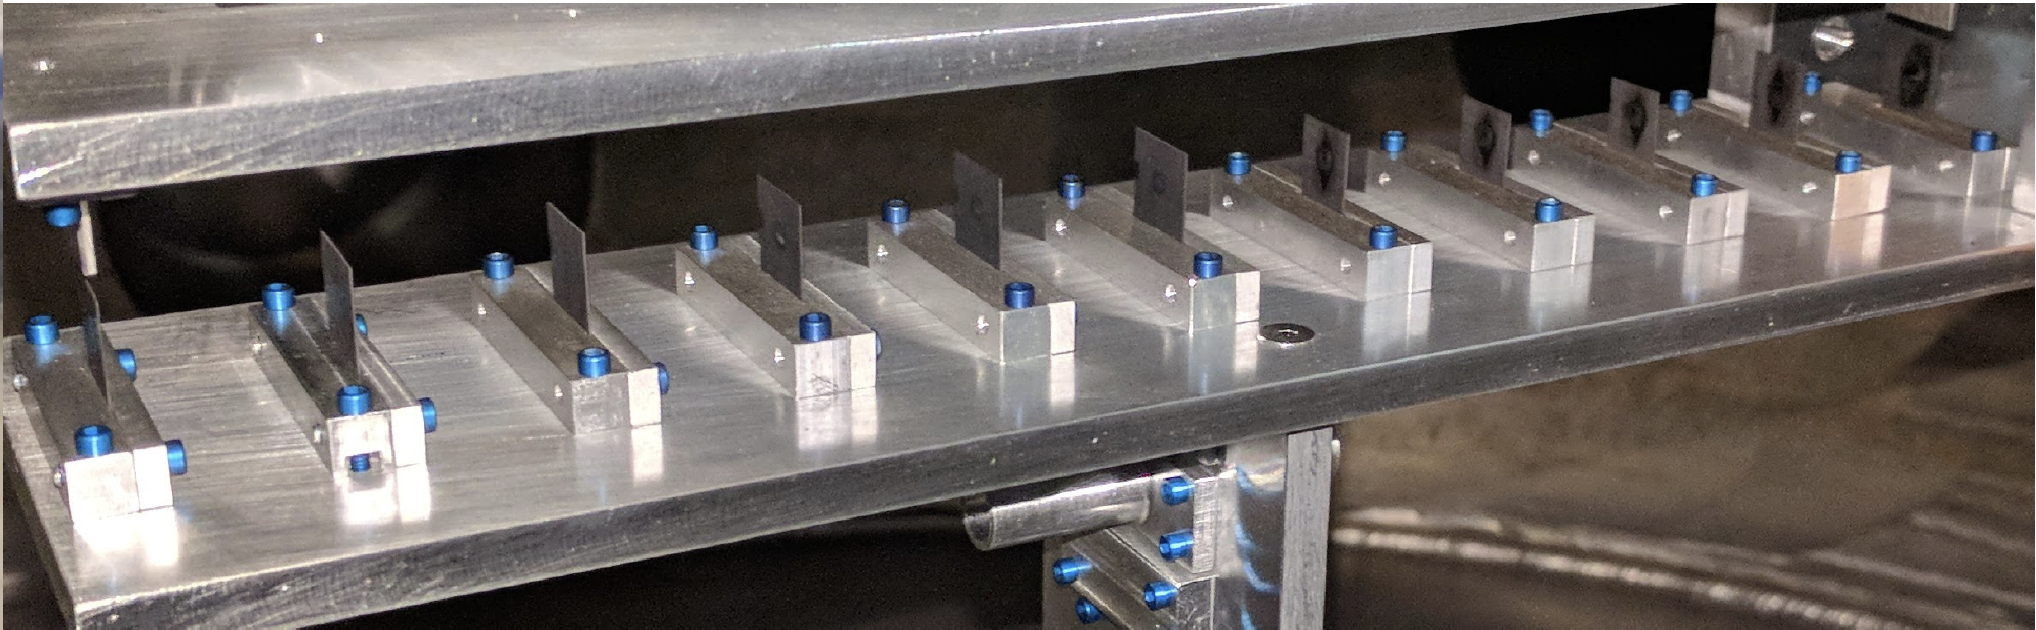
\includegraphics[width=0.2\textwidth] {./optics_plot/optics_3.png}
 		\caption{Mutifoil Target for Tritium Experiment: 11 carbon foil totally which can cover the full 25cm target length} \label{optics_plt2}
 	\end{center}
\end{figure}   

\begin{figure}
 	\begin{center}
 		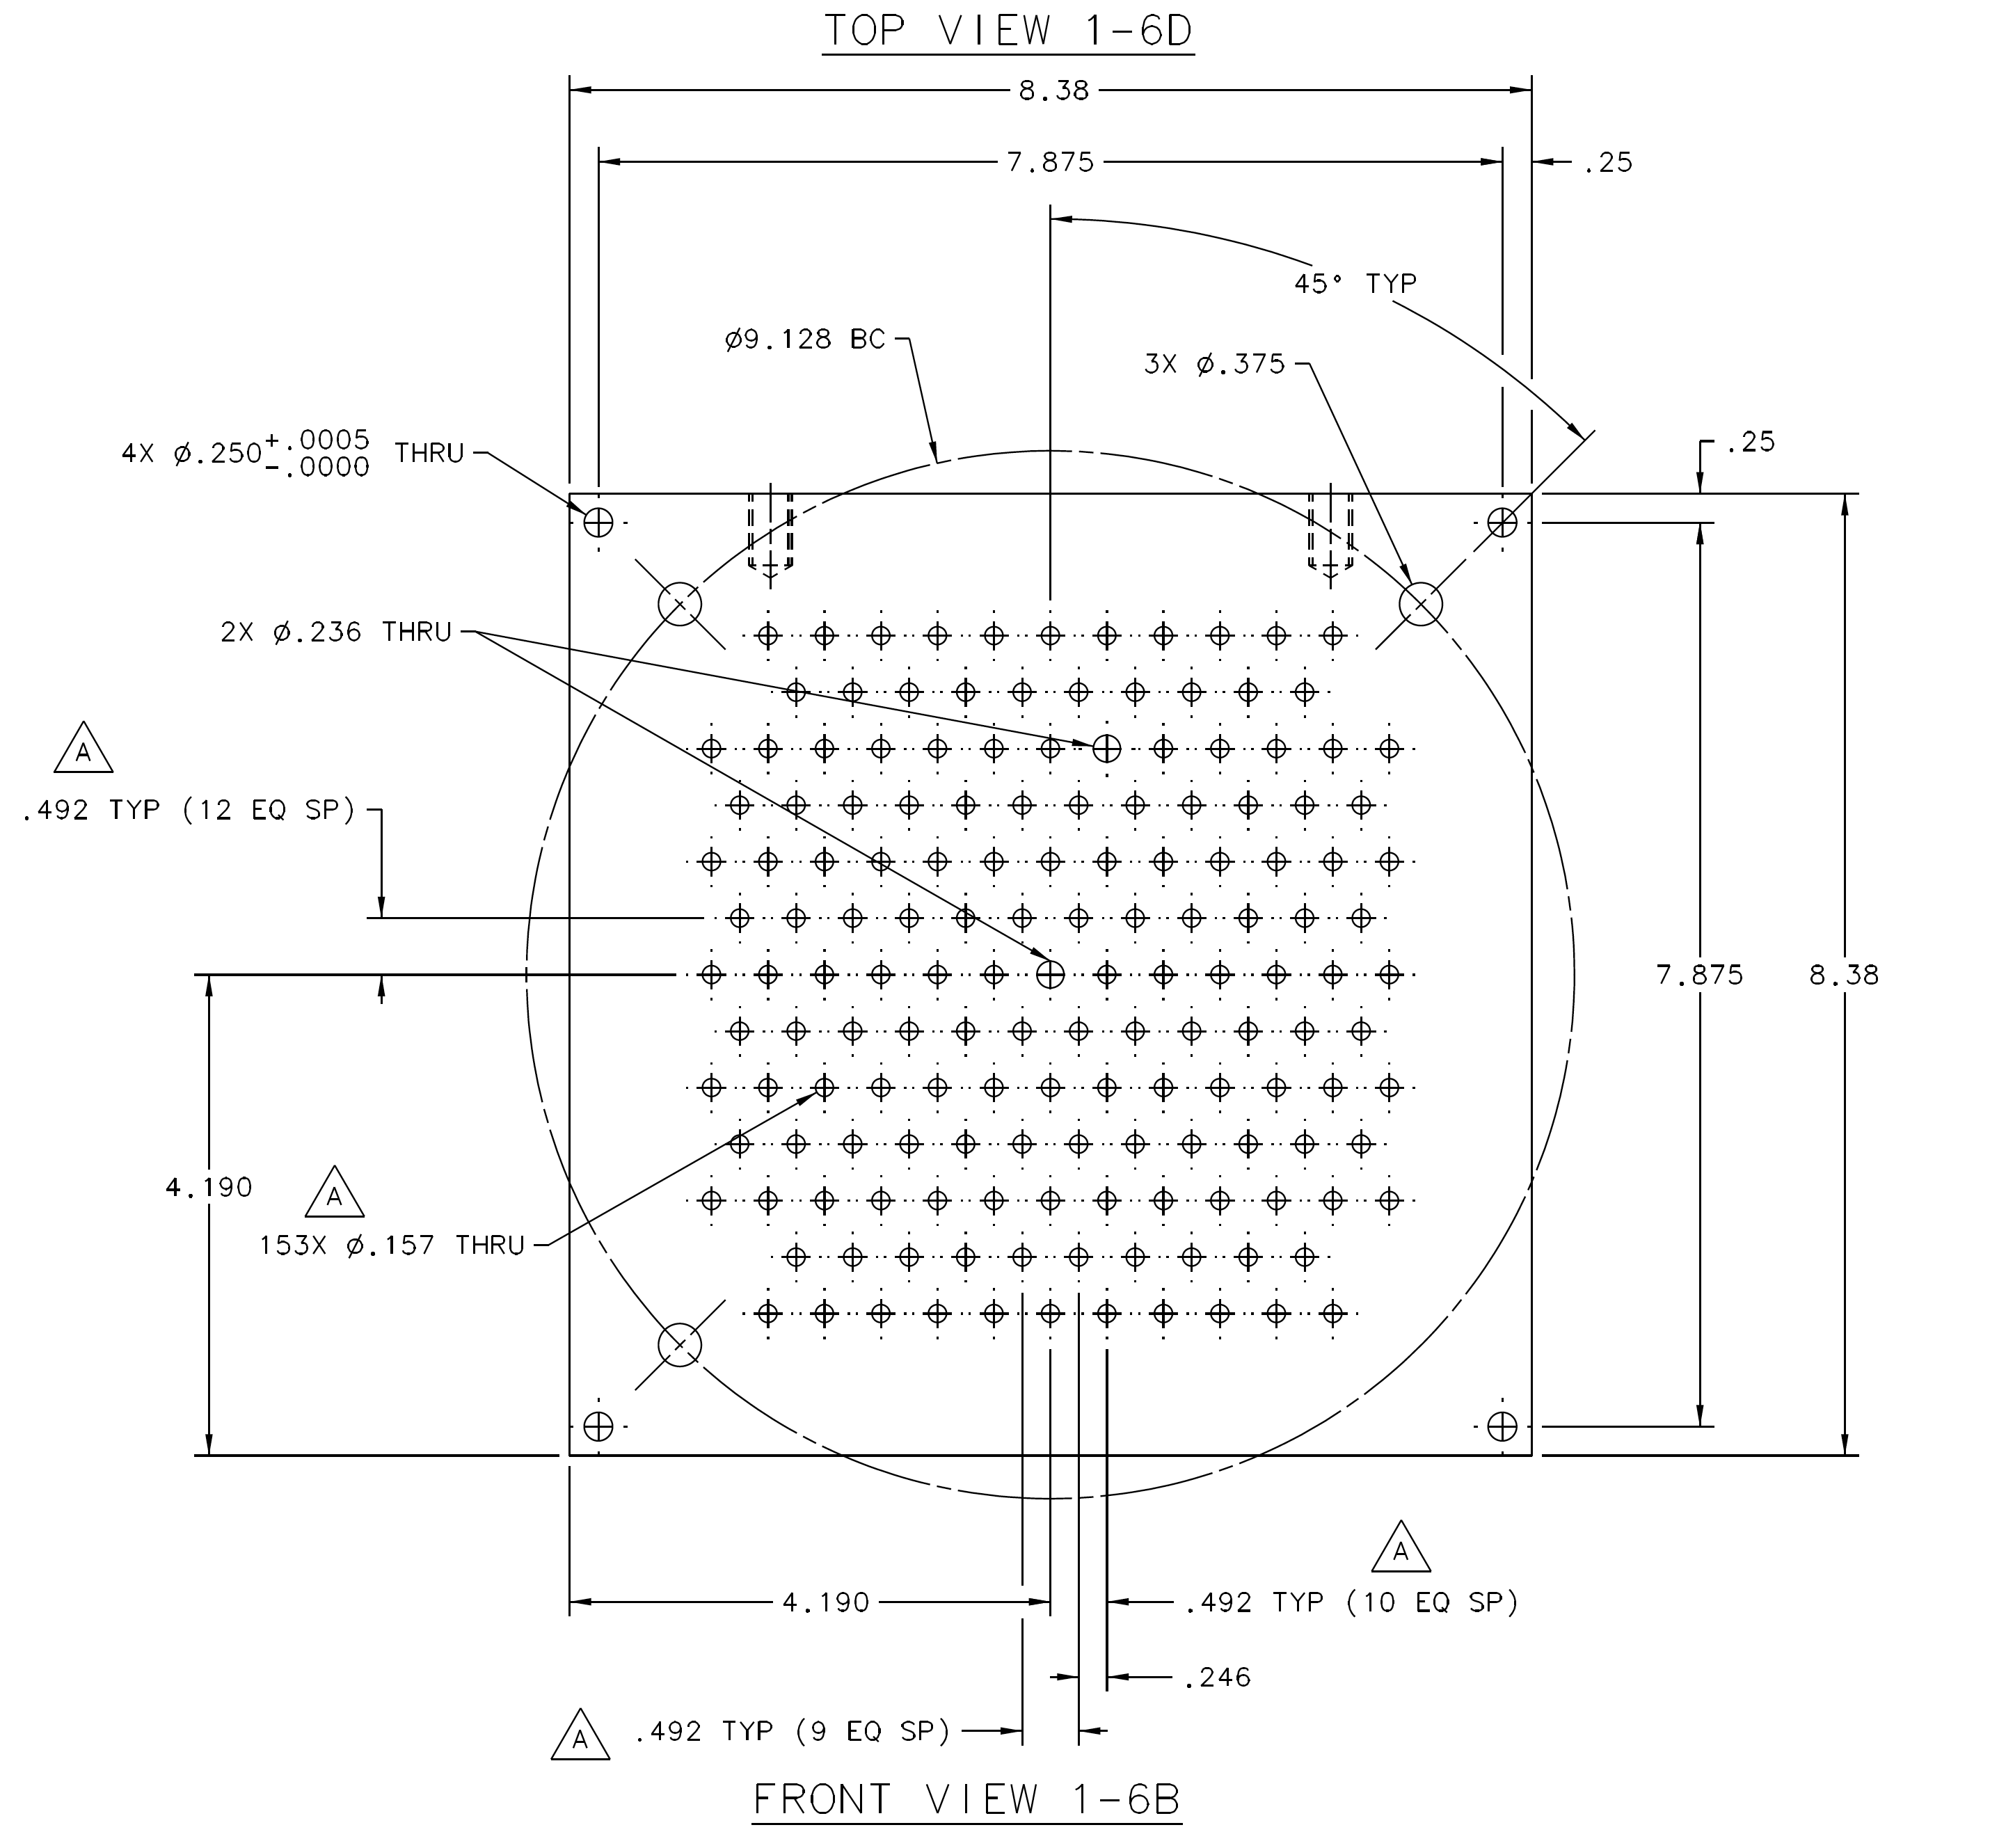
\includegraphics[width=0.2\textwidth] {./optics_plot/optics_1.png}
 		\caption{Engineering schematic plot for sieve-slit collimator used for Tritium Experiment } \label{optics_plt3}
 	\end{center}
\end{figure}   
For the three spatial target variable optimization, firstly, good events need to be selected by apply the general good electron cut and then for each selected event, which foil it is scattered from the target($Foil\_id$) and which hole it passes through the 
sleve-silt($Holel\_id$) need to be discriminated. Combining with all the positions mentioned above, the really target variable $y_{tg}^{REAL}$, $\theta_{tg}^{REAL}$ and $\phi_{tg}^{REAL}$ can be calculated by the geometrical relationships. On the other side, from the initial optics matrix which usually comes from the pervious experiment the reconstructed target variables: $y_{tg}^{RCON}$, $\theta_{tg}^{RCON}$ and $\phi_{tg}^{RCON}$ can be obtained. Then the optics matrix elements can be optimized by minimizing the following aberration funtion:
\begin{equation}  
\Delta(O)=\sum_{events}\left( O^{RECON}-O^{REAL}\right) ^{2}
\end{equation} \label{optics_3}  
Where $O$ stands the $y_{tg}$, $\theta_{tg}$ and $\phi_{tg}$ 

The momentum optimization is similar. After selecting out the elastic scattering events, for each event , the $\delta_{tg}^{RCON}$ and $\delta_{tg}^{REAL}$ can be obtained and optics matrix elements can be optimized by the Eq \ref{optics_3}. But usually to precisely determined the scattering momentum, several corrections need to be applied such as a variety of the energy loss and the elastic peak shift within the spectrometer acceptance. 


\section{Result}
For MARATHON experiment, all the production data was taken at spring,2018  when the HRS magnets tuning was exactly same with the previous GMP experiment so that our magnets optics is also same with the GMP one.  We keep using the GMP most updated optics matrix for both HRS and base on our online check no obvious abnormity found for that GMP optics matrix

MARATHON also use some data about target density study (Boiling effect) taken at Fall,2017. This data used a slliently different tuning than the GMP experiment. Therefore optics for that part of data is analyzed . Since only optics data related to the spatial variable was taken so only $y_{tg}$, $\theta_{tg}$ and $\phi_{tg}$ are optimized and some reault are shown in the Fig \ref{optics_plt4}, Fig \ref{optics_plt5} and Fig \ref{optics_plt6}


\begin{figure}[htbp]
\subfigure[before calibration]{
\begin{minipage}[t]{1\linewidth}
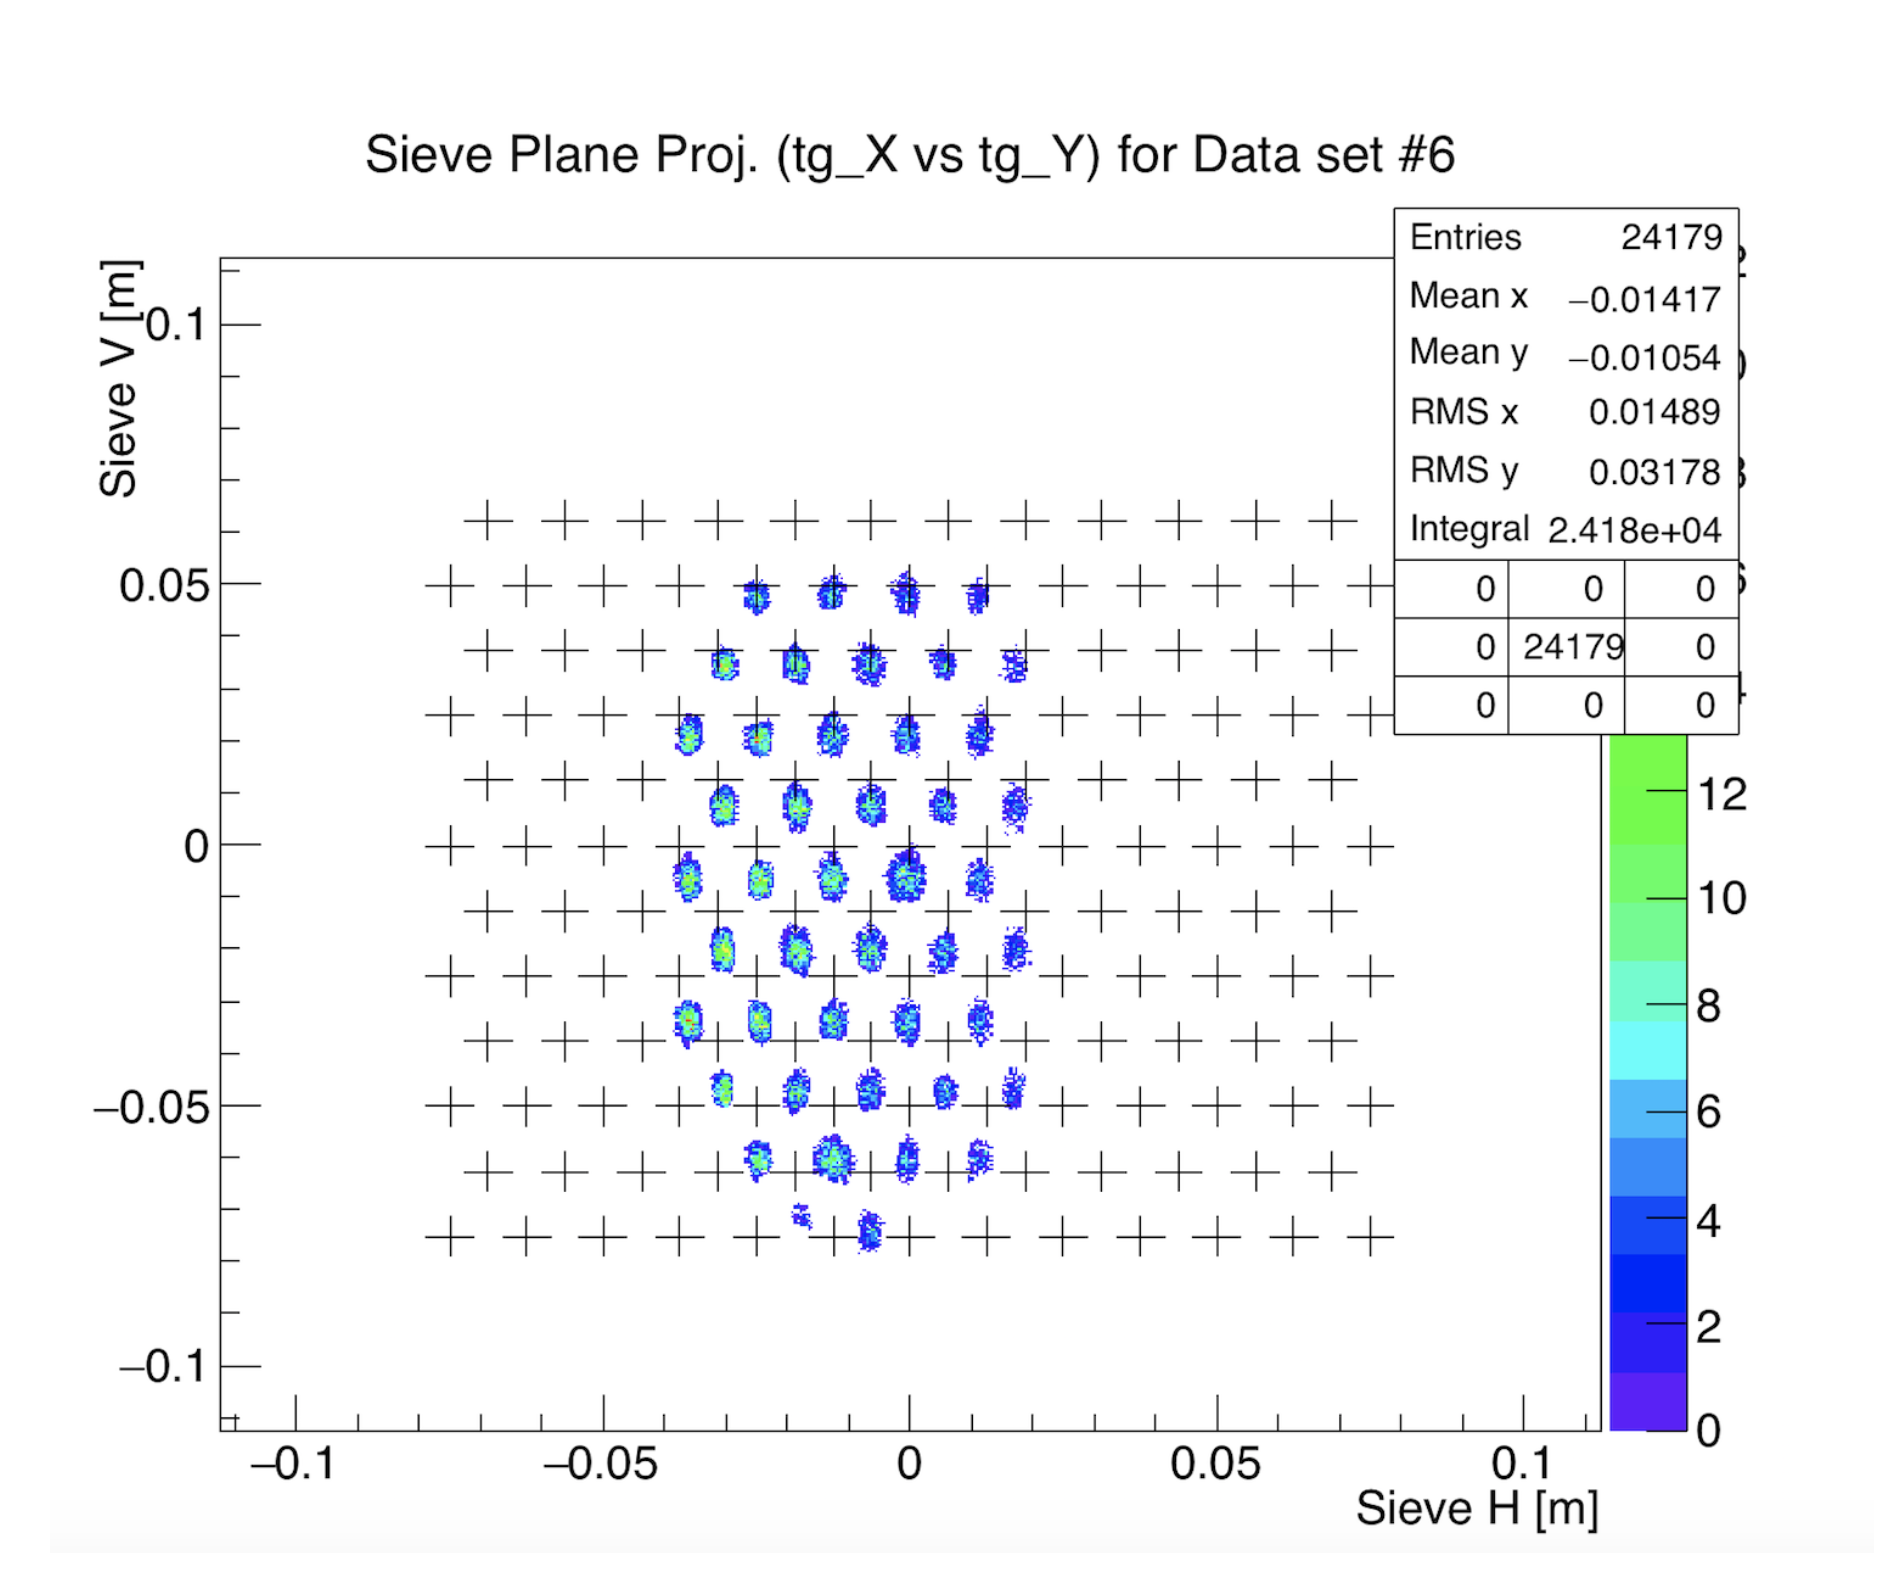
\includegraphics[width=3in]{./optics_plot/optics_6.png}
\end{minipage}
}\\
\subfigure[after calibration]{
\begin{minipage}[t]{1\linewidth}
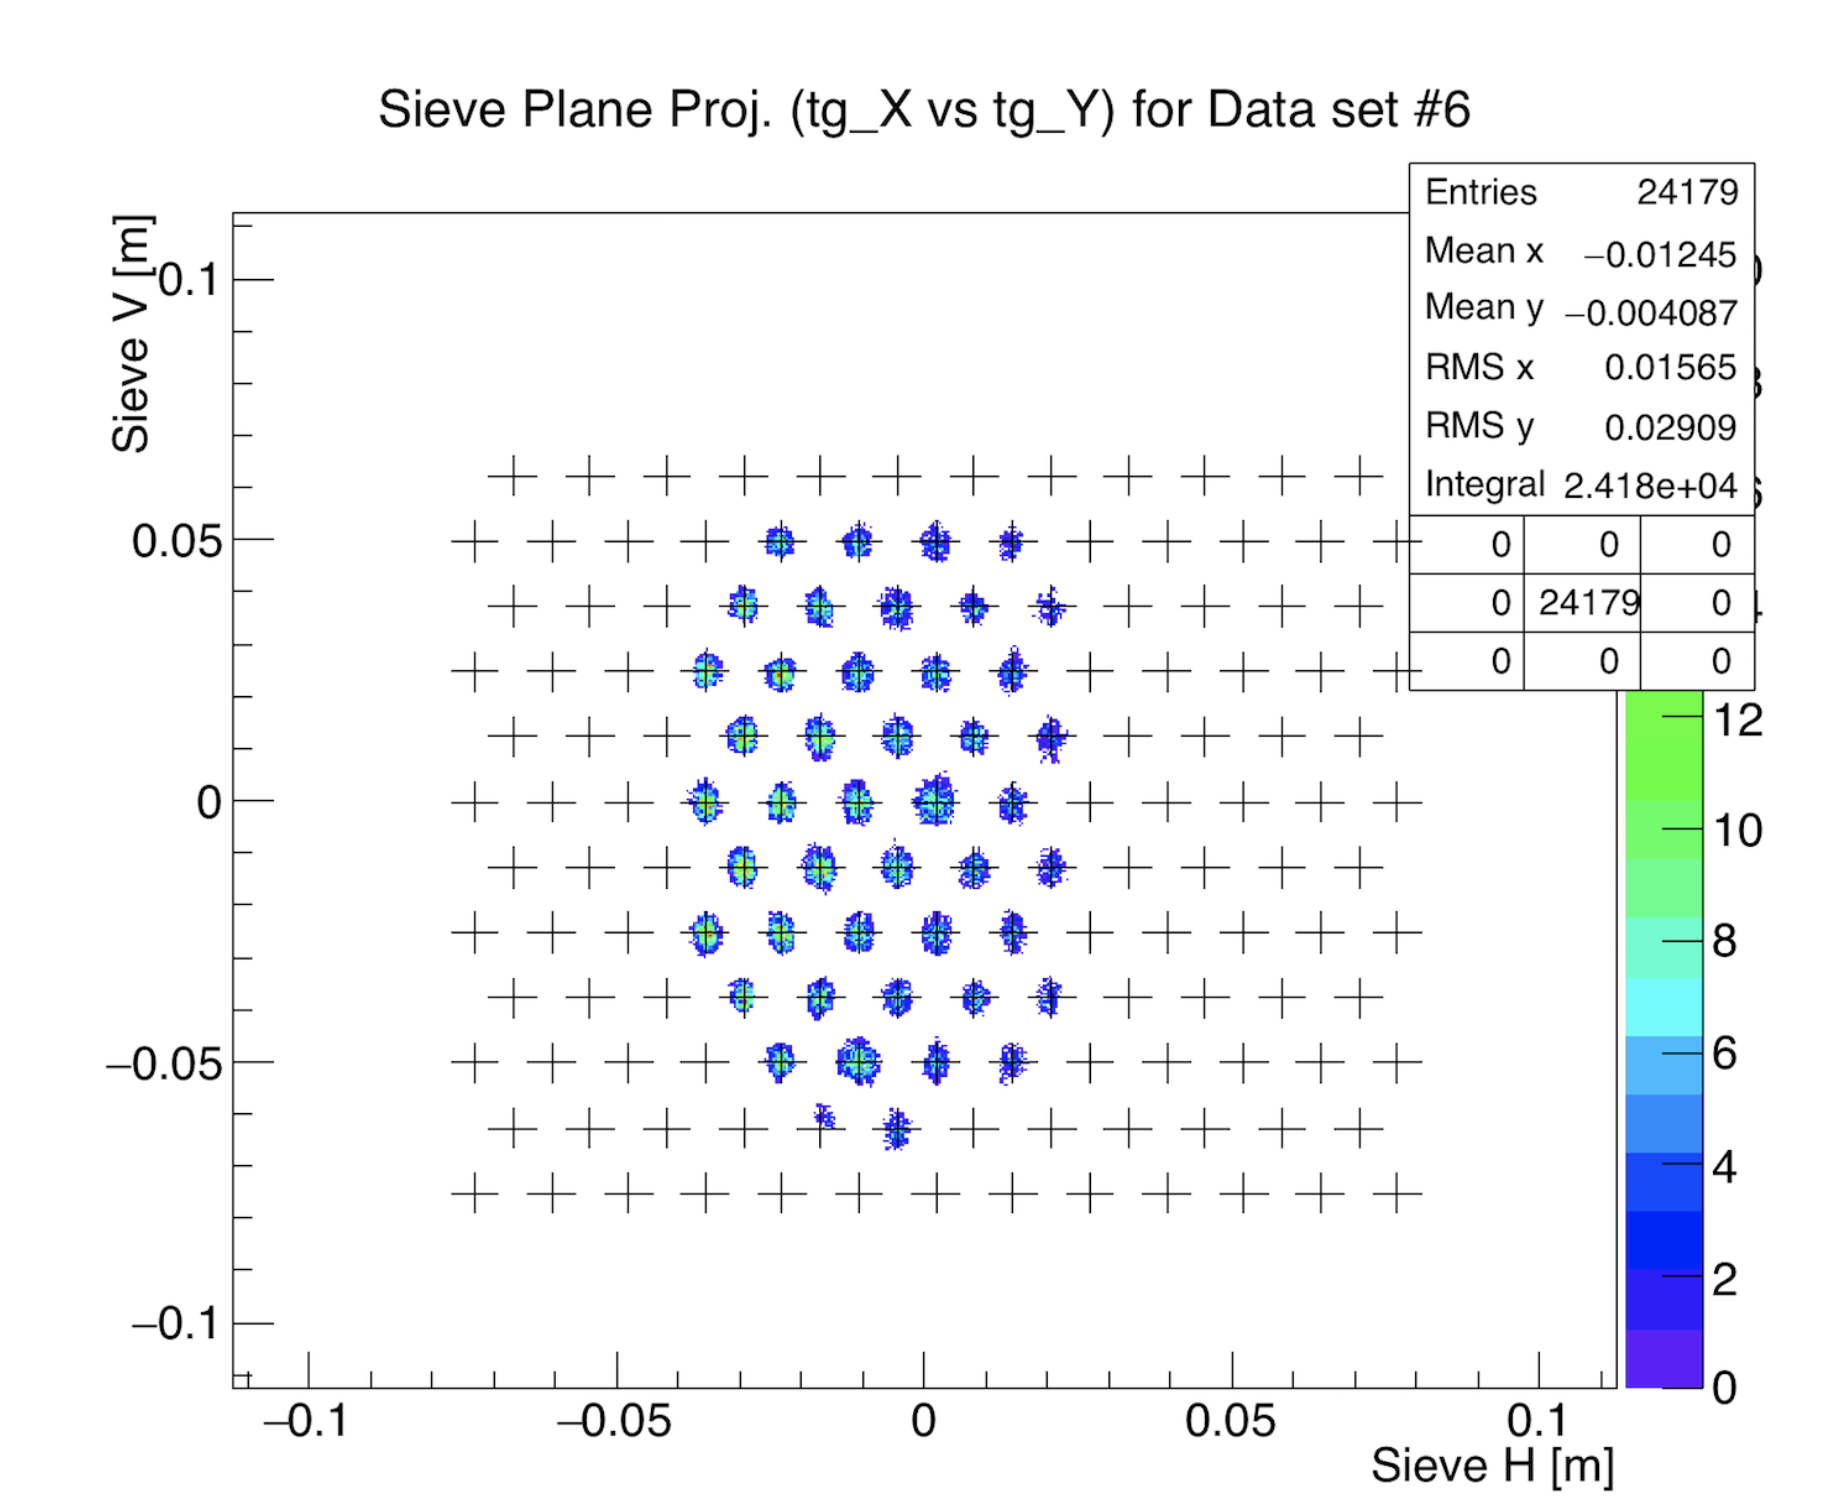
\includegraphics[width=3in]{./optics_plot/optics_5.png}
\end{minipage}
}
 \centering
\caption{$\theta_{tg} $ and $\phi_{tg}$ calibration for the fall,2017 data}
\label{optics_plt4}
\end{figure}

\begin{figure}[htbp]
\subfigure[before calibration]{
\begin{minipage}[t]{1\linewidth}
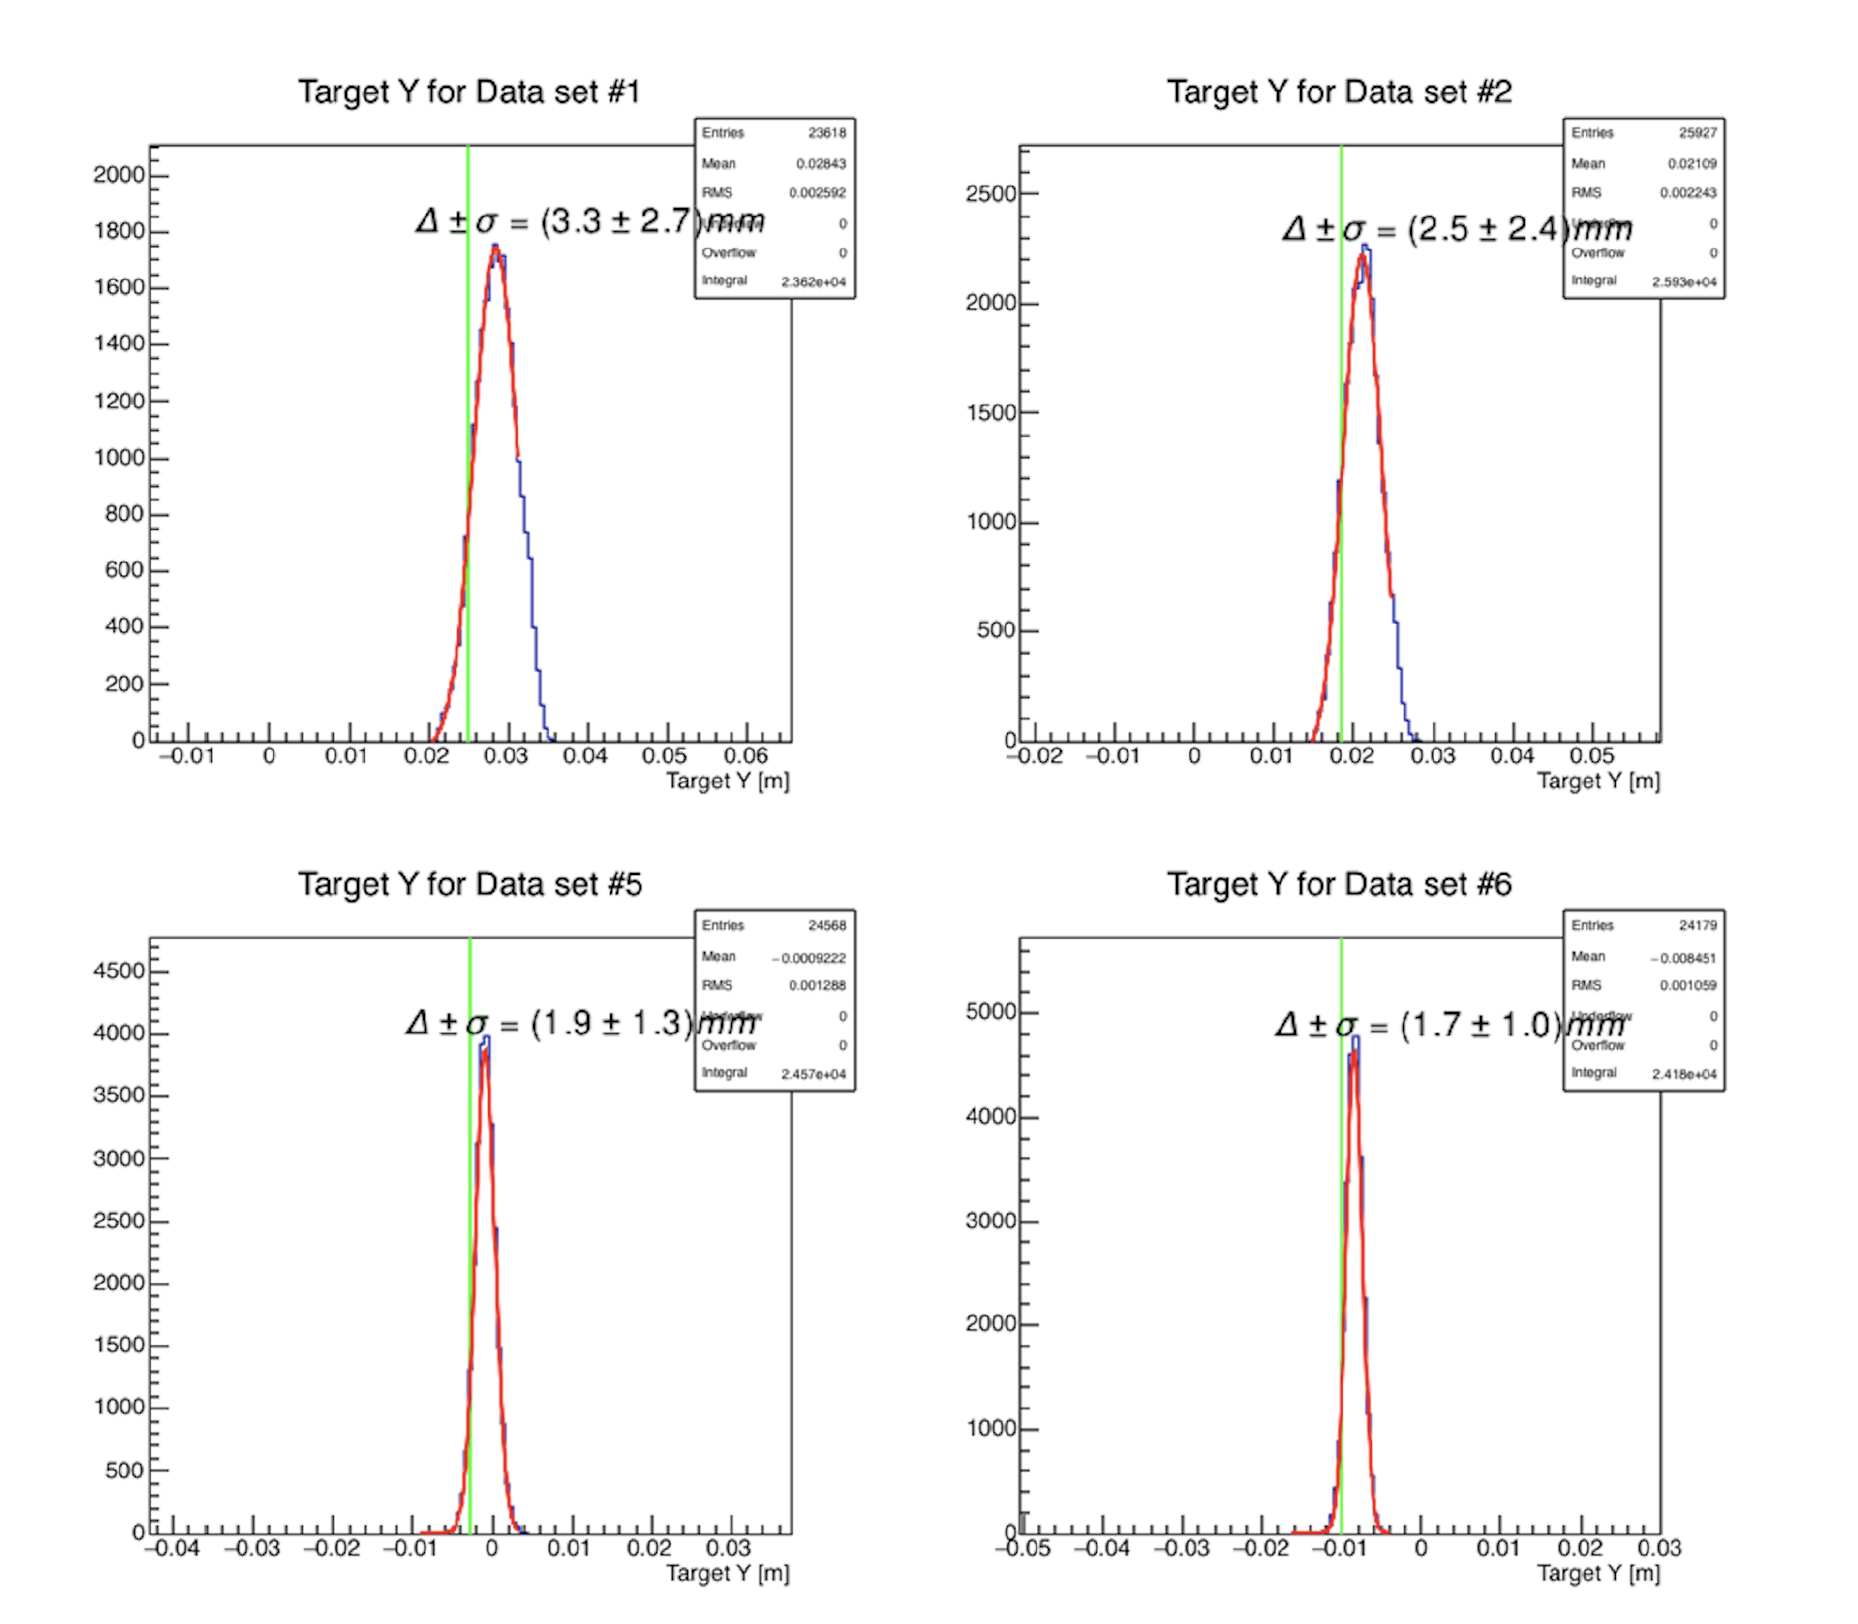
\includegraphics[width=3in]{./optics_plot/optics_8.png}
\end{minipage}
}\\
\subfigure[after calibration]{
\begin{minipage}[t]{1\linewidth}
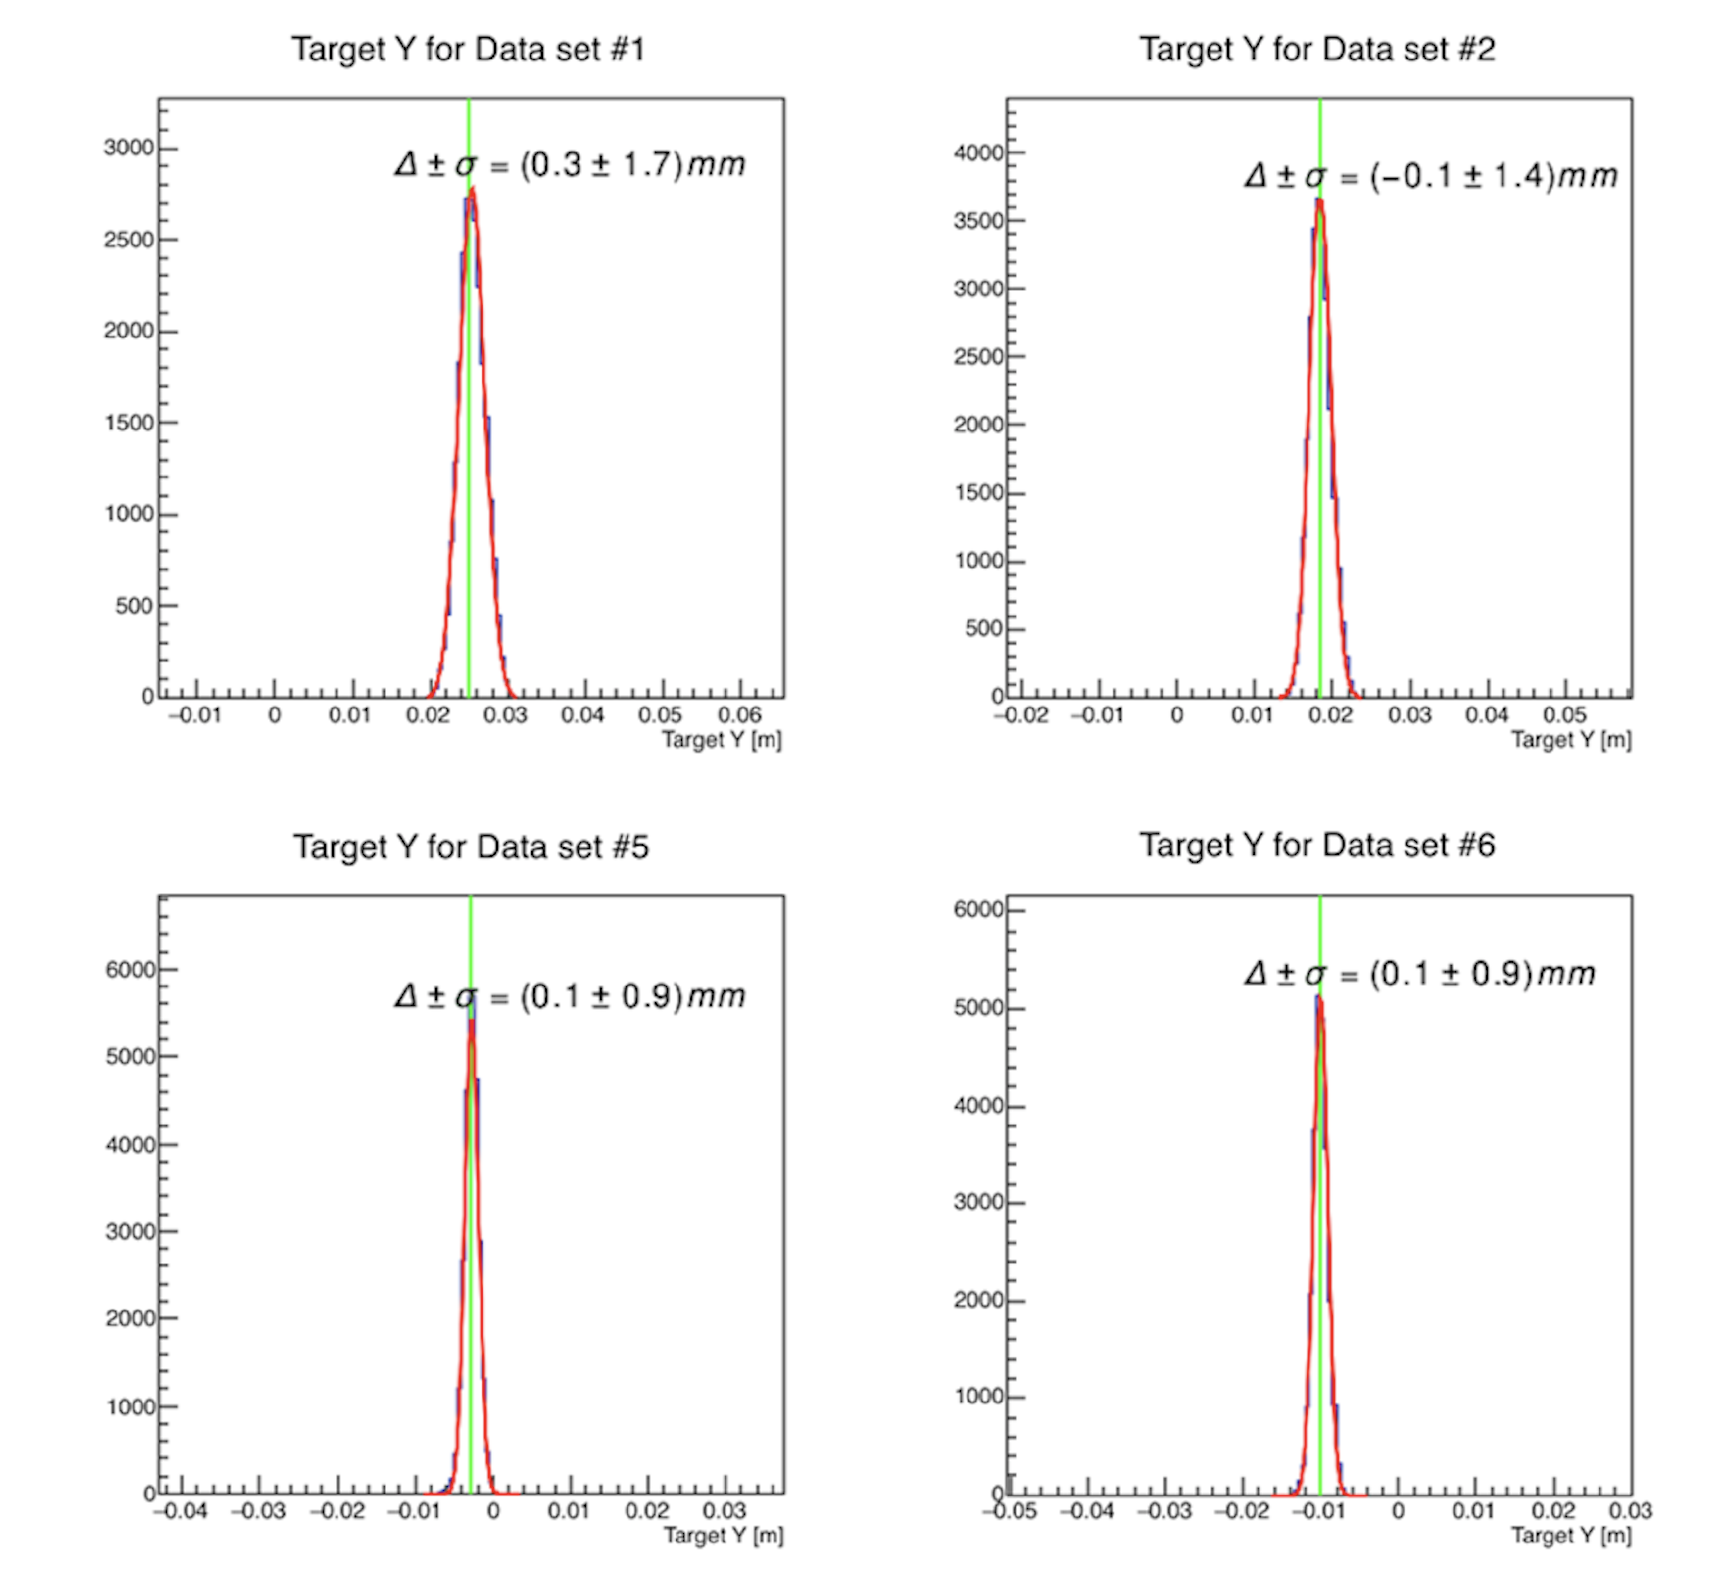
\includegraphics[width=3in]{./optics_plot/optics_7.png}
\end{minipage}
}
 \centering
\caption{$y_{tg}$ calibration for the fall,2017 data}
\label{optics_plt5}
\end{figure}

\begin{figure}
 	\begin{center}
 		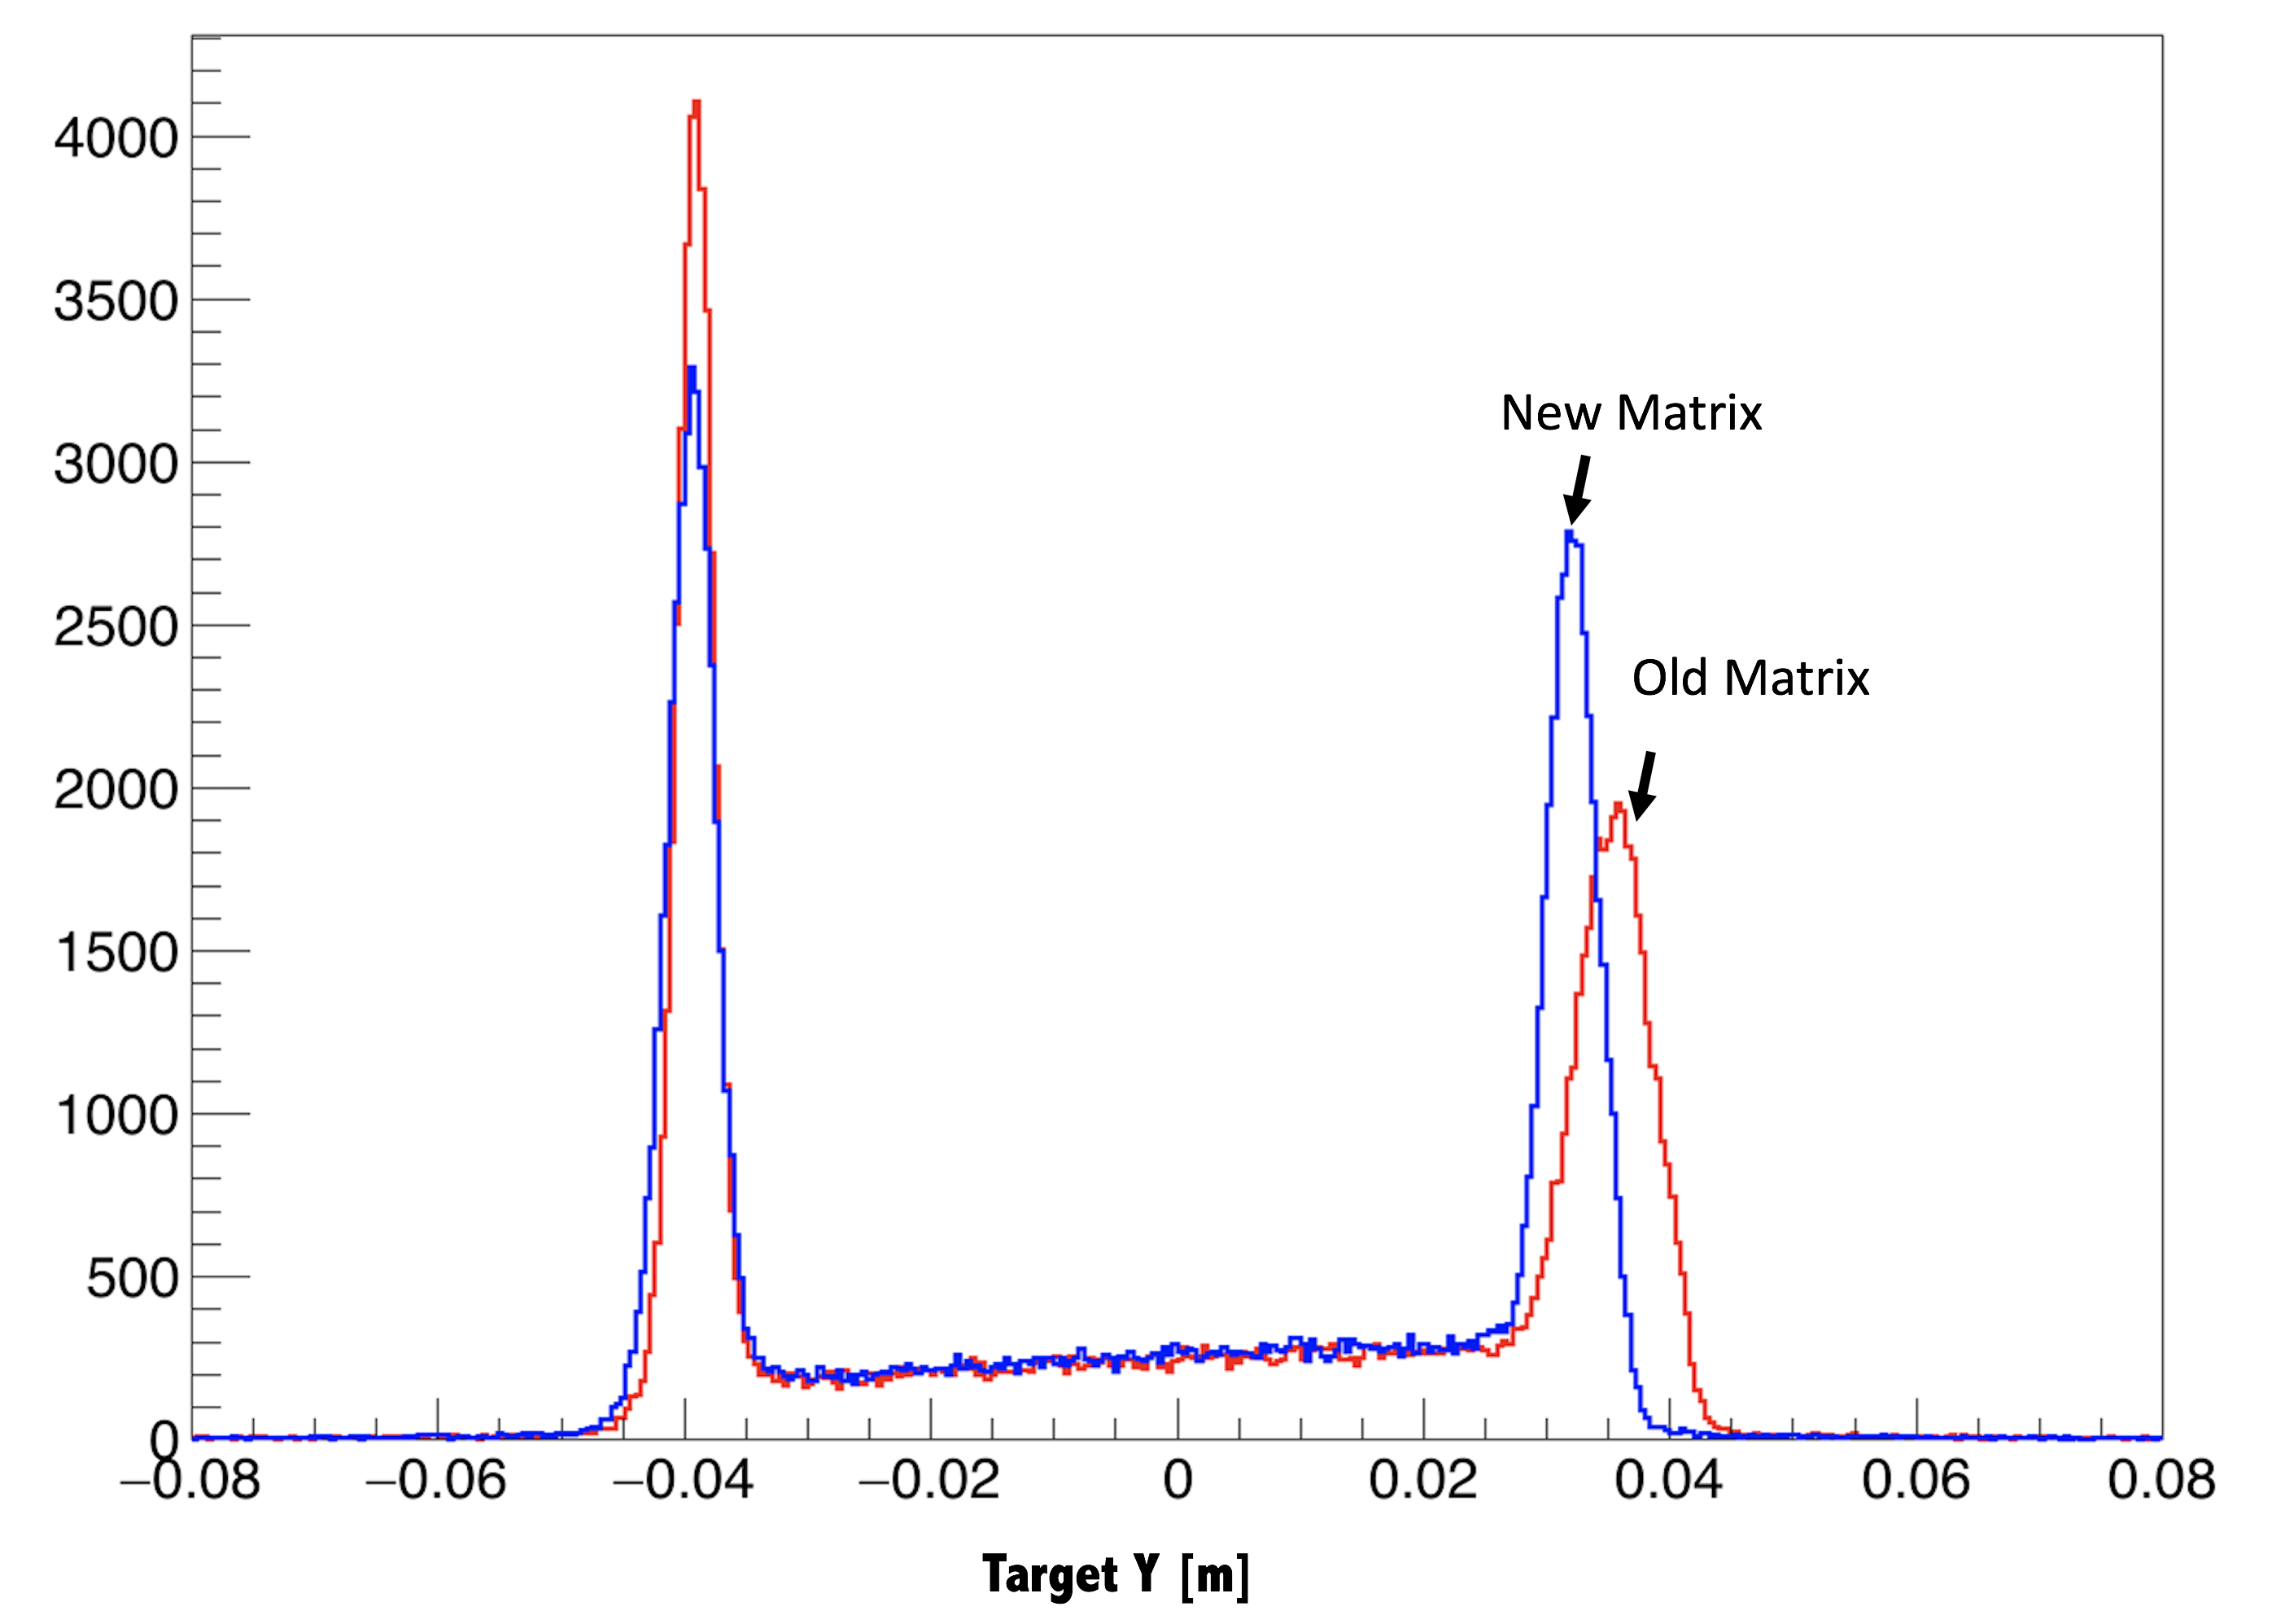
\includegraphics[width=0.3\textwidth] {./optics_plot/optics_2.png}
 		\caption{$y_{tg}$ reconstruction before and after optimize the optice matrix, as we can see , the upstream endcap resolution become better} \label{optics_plt6}
 	\end{center}
\end{figure}   
